\documentclass[11pt,a4paper]{article}

% ── Packages ──────────────────────────────────────────────
\usepackage[utf8]{inputenc}
\usepackage[T1]{fontenc}
\usepackage{mathpazo}              % Palatino — readable, academic
\usepackage[margin=2.5cm]{geometry}
\usepackage{graphicx}
\usepackage{booktabs}
\usepackage{hyperref}
\usepackage{xcolor}
\usepackage{enumitem}
\usepackage{float}
\usepackage{tikz}
\usepackage{pgfplots}
\pgfplotsset{compat=1.18}
\usepackage{caption}
\usepackage{listings}
\usepackage{fancyvrb}
\usepackage[style=numeric,sorting=nyt,backend=biber]{biblatex}

\hypersetup{
  colorlinks=true,
  linkcolor=blue!60!black,
  citecolor=blue!60!black,
  urlcolor=blue!60!black,
}

\lstset{
  basicstyle=\ttfamily\small,
  keywordstyle=\color{blue!70!black},
  commentstyle=\color{green!50!black},
  stringstyle=\color{red!60!black},
  frame=single,
  framerule=0.4pt,
  rulecolor=\color{gray!50},
  backgroundcolor=\color{gray!5},
  breaklines=true,
  showstringspaces=false,
  tabsize=4,
  language=Python,
}

% ── Bibliography ──────────────────────────────────────────
\usepackage{filecontents}
\begin{filecontents}{\jobname.bib}
@article{Karr2012,
  author  = {Karr, Jonathan R. and Sanghvi, Jayodita C. and Macklin, Derek N.
             and Gutschow, Miriam V. and Jacobs, Jared M. and Bolival, Benjamin
             and Assad-Garcia, Nacyra and Glass, John I. and Covert, Markus W.},
  title   = {A whole-cell computational model predicts phenotype from genotype},
  journal = {Cell},
  year    = {2012},
  volume  = {150},
  number  = {2},
  pages   = {389--401},
  doi     = {10.1016/j.cell.2012.05.044},
}
@article{Sun2021,
  author  = {Sun, Gwanggyu and Ahn-Horst, Travis A. and Covert, Markus W.},
  title   = {The \textit{E.~coli} whole-cell modeling project},
  journal = {EcoSal Plus},
  year    = {2021},
  volume  = {9},
  number  = {2},
  pages   = {eESP-0001-2020},
  doi     = {10.1128/ecosalplus.ESP-0001-2020},
}
@article{AhnHorst2022,
  author  = {Ahn-Horst, Travis A. and Mille, Luis Santiago and Sun, Gwanggyu
             and Morrison, Jerry H. and Covert, Markus W.},
  title   = {An expanded whole-cell model of \textit{E.~coli} links cellular
             physiology with mechanisms of growth rate control},
  journal = {npj Systems Biology and Applications},
  year    = {2022},
  volume  = {8},
  number  = {1},
  pages   = {30},
  doi     = {10.1038/s41540-022-00242-9},
}
@article{Choi2023,
  author  = {Choi, Heejo and Covert, Markus W.},
  title   = {Whole-cell modeling of \textit{E.~coli} confirms that
             in~vitro tRNA aminoacylation measurements are insufficient
             to support cell growth},
  journal = {Nucleic Acids Research},
  year    = {2023},
  volume  = {51},
  number  = {12},
  pages   = {5911--5930},
  doi     = {10.1093/nar/gkad435},
}
@article{Scott2010,
  author  = {Scott, Matthew and Gunderson, Carl W. and Mateescu, Eduard M.
             and Zhang, Zhongge and Hwa, Terence},
  title   = {Interdependence of cell growth and gene expression: origins
             and consequences},
  journal = {Science},
  year    = {2010},
  volume  = {330},
  number  = {6007},
  pages   = {1099--1102},
  doi     = {10.1126/science.1192588},
}
@article{Hoops2006,
  author  = {Hoops, Stefan and Sahle, Sven and Gauges, Ralph and Lee, Christine
             and Pahle, J{\"u}rgen and Simus, Natalia and Singhal, Mudita
             and Xu, Liang and Mendes, Pedro and Kummer, Ursula},
  title   = {{COPASI} --- a {CO}mplex {PA}thway {SI}mulator},
  journal = {Bioinformatics},
  year    = {2006},
  volume  = {22},
  number  = {24},
  pages   = {3067--3074},
  doi     = {10.1093/bioinformatics/btl485},
}
@article{Moraru2008,
  author  = {Moraru, Ion I. and Schaff, James C. and Slepchenko, Boris M.
             and Blinov, Michael L. and Morgan, Frank and Lakshminarayana, Anu
             and Gao, Fei and Li, Ye and Loew, Leslie M.},
  title   = {Virtual {Cell} modelling and simulation software environment},
  journal = {IET Systems Biology},
  year    = {2008},
  volume  = {2},
  number  = {5},
  pages   = {352--362},
  doi     = {10.1049/iet-syb:20080102},
}
@article{Skalnik2023,
  author  = {Skalnik, Christopher J. and Cheah, Sean Y. and Yang, Mica Y.
             and Wolff, Mattheus B. and Spangler, Ryan K. and Talman, Lee
             and Morrison, Jerry H. and Peirce, Shayn M. and Agmon, Eran
             and Covert, Markus W.},
  title   = {Whole-cell modeling of \textit{E.~coli} colonies enables
             quantification of single-cell heterogeneity in antibiotic
             responses},
  journal = {PLOS Computational Biology},
  year    = {2023},
  volume  = {19},
  number  = {6},
  pages   = {e1011232},
  doi     = {10.1371/journal.pcbi.1011232},
}
@article{Burkhart2012,
  author  = {Burkhart, Julia M. and Vaudel, Marc and Gambaryan, Stepan
             and Radau, Stefanie and Walter, Ulrich and Martens, Lennart
             and Geiger, J{\"o}rg and Sickmann, Albert and Zahedi, Ren{\'e} P.},
  title   = {The first comprehensive and quantitative analysis of human
             platelet protein composition allows the comparative analysis
             of structural and functional pathways},
  journal = {Blood},
  year    = {2012},
  volume  = {120},
  number  = {15},
  pages   = {e73--e82},
  doi     = {10.1182/blood-2012-04-416594},
}
@article{Purvis2008,
  author  = {Purvis, J. E. and Chatterjee, M. S. and Brass, L. F.
             and Diamond, S. L.},
  title   = {A molecular signaling model of platelet phosphoinositide
             and calcium regulation during homeostasis and {P2Y1} activation},
  journal = {Blood},
  year    = {2008},
  volume  = {112},
  number  = {10},
  pages   = {4069--4079},
  doi     = {10.1182/blood-2008-05-157883},
}
\end{filecontents}
\addbibresource{\jobname.bib}

% ── Title ─────────────────────────────────────────────────
\title{%
  \Large Whole-Cell Modelling of \textit{E.~coli} \\[4pt]
  \large Architecture, Web Interface, and \\
         a Proposed Extension to Human Platelets \\[10pt]
  \normalsize \textit{Project Report}
}
\author{Steve Haigh}
\date{March 2026}

\begin{document}
\maketitle
\thispagestyle{empty}
\tableofcontents
\newpage


% ══════════════════════════════════════════════════════════
\part{The Model}
% ══════════════════════════════════════════════════════════

% ──────────────────────────────────────────────────────────
\section{Introduction}
% ──────────────────────────────────────────────────────────

Most computational models in biology focus on one pathway or one organelle at
a time.  A \emph{whole-cell model} tries something more ambitious: it
simulates every known process inside a living cell, all running
simultaneously, so that the emergent behaviour of the whole organism can be
studied rather than the behaviour of its parts in isolation.

The first such model, published in 2012 by Karr and colleagues at Stanford
University, simulated the complete life cycle of \textit{Mycoplasma
genitalium}~\cite{Karr2012}.  The same group --- the Covert Lab --- has since
built a much larger whole-cell model of \textit{Escherichia
coli}~\cite{Sun2021, AhnHorst2022}, incorporating roughly 43\% of that
organism's characterised genes.  This model, called \textbf{wcEcoli}, is
open-source and publicly available.

The wcEcoli model has been used to study growth-rate
control~\cite{AhnHorst2022}, tRNA charging dynamics~\cite{Choi2023}, and
antibiotic heterogeneity in colonies~\cite{Skalnik2023}.

This report provides an overview of the wcEcoli model --- what it does, how it
works, and what its output looks like --- together with a description of the
browser-based user interface I have built to make the model easier to use.
Finally, and most importantly, it outlines a proposed extension of the
modelling framework to simulate \emph{human platelets}.

If you are familiar with tools such as COPASI~\cite{Hoops2006} or Virtual
Cell~\cite{Moraru2008}, it may help to start with the differences.  COPASI
and VCell each model a chosen set of reactions: you define the species, write
rate laws, and the software integrates the differential equations.  wcEcoli
does not ask you to write equations.  Instead, its authors have already
encoded 17 distinct biological processes --- metabolism, transcription,
translation, DNA replication, cell division, and so on --- each using whatever
mathematical technique suits it best (flux-balance analysis for metabolism,
stochastic kinetics for gene regulation, ordinary differential equations for
tRNA charging, and others).

Could a whole-cell model be built in COPASI instead?  In principle, COPASI can
handle large ODE and stochastic systems, but in practice the approach runs into
several difficulties.  COPASI represents a model as a single network of
reactions and species; there is no built-in mechanism for mixing mathematical
formalisms within one simulation --- for example, combining flux-balance
analysis for metabolism with stochastic kinetics for gene regulation and ODEs
for tRNA charging, as wcEcoli does.  A user would have to force every process
into one formalism or manage multiple COPASI models externally and synchronise
their states at each timestep, which would negate much of the tool's
convenience.  Performance is also a concern: COPASI's general-purpose ODE
integrators scale poorly beyond a few thousand species, whereas wcEcoli tracks
tens of thousands of molecular species and individually resolved macromolecules
(each ribosome, each replication fork) at one-second resolution for an entire
cell cycle.  The wcEcoli framework achieves this by using specialised solvers
for each process and a custom integer-partitioning scheme for resource
allocation --- optimisations that a general-purpose tool cannot easily
replicate.  COPASI remains an excellent choice for pathway-scale models, but the
architectural demands of whole-cell modelling --- heterogeneous formalisms,
discrete molecule tracking, and tight coupling between dozens of concurrent
processes --- call for a purpose-built engine.


% ──────────────────────────────────────────────────────────
\section{What the Model Does}
% ──────────────────────────────────────────────────────────

Every second of simulated time, each of the 17 processes declares what
molecules it needs, receives an allocation from a shared pool, and then
updates the state of the cell.  The result is a simulation that
tracks \emph{individual molecules}: individual ribosomes translating
individual mRNAs; individual replication forks progressing along the
chromosome.  A typical simulation covers one full cell cycle (roughly 25--130
minutes, depending on the growth condition) and produces a detailed trace of
every measurable quantity along the way.

\subsection{What goes in}

The model is parameterised from roughly 80 curated data files drawn from
experimental literature and databases such as EcoCyc.  A preprocessing step
called the \emph{Parameter Calculator} (ParCa) reads these raw data and fits
them into a consistent set of initial conditions and rate constants.  This
step takes about 18 minutes on a modern laptop and needs to be run only once
per set of conditions.

\subsection{What comes out}

The simulation produces time-series data for every tracked quantity at
one-second resolution.  There are over 80 built-in analysis scripts that
generate publication-quality plots from this output.  Among the most commonly
examined are:

\begin{itemize}[nosep]
  \item \textbf{Cell mass over time} --- dry mass, protein mass, RNA mass,
        DNA mass, and their fractions.
  \item \textbf{Metabolic fluxes} --- central carbon metabolism, amino acid
        exchange rates, glucose yield.
  \item \textbf{Gene expression} --- mRNA counts, protein counts, ribosome
        and RNA polymerase occupancy.
  \item \textbf{DNA replication} --- replication fork position, replisome
        counts, origin firing.
  \item \textbf{Growth-rate determinants} --- tRNA charging levels, ppGpp
        concentration, ribosomal capacity.
\end{itemize}

\subsection{Growth conditions and variants}

The model ships with five named growth conditions:

\begin{table}[H]
\centering
\caption{Built-in growth conditions.}
\begin{tabular}{llc}
  \toprule
  \textbf{Name} & \textbf{Carbon source / supplements} & \textbf{Doubling time} \\
  \midrule
  \texttt{basal}       & Glucose minimal                & $\sim$44 min \\
  \texttt{with\_aa}    & Glucose + all 20 amino acids   & $\sim$25 min \\
  \texttt{acetate}     & Acetate minimal                & $\sim$136 min \\
  \texttt{succinate}   & Succinate minimal              & $\sim$82 min \\
  \texttt{no\_oxygen}  & Glucose minimal, anaerobic     & $\sim$100 min \\
  \bottomrule
\end{tabular}
\end{table}

Beyond fixed conditions, the \emph{timelines} variant system allows media
shifts at arbitrary times during a simulation.  Twenty-nine pre-defined
timelines cover nutrient upshifts, downshifts, carbon-source switches, and
transitions to anaerobic growth.


% ──────────────────────────────────────────────────────────
\section{An Example: Minimal vs.\ Rich Media}
\label{sec:example}
% ──────────────────────────────────────────────────────────

To illustrate what the model can do, consider a comparison between two growth
conditions.  In \textbf{minimal glucose media}, the cell must synthesise all
20 amino acids and every other building block from glucose and salts.  In
\textbf{rich media} (glucose supplemented with all 20 amino acids), the cell
can import amino acids directly and redirect its resources.

This comparison recapitulates one of the best-known results in bacterial
physiology: the ``growth law'' described by Scott et al.~\cite{Scott2010},
which states that the fraction of the cell devoted to ribosomes scales
linearly with growth rate.  The wcEcoli model reproduces this relationship
as an emergent property, not as a built-in assumption~\cite{AhnHorst2022}.

\begin{figure}[H]
\centering
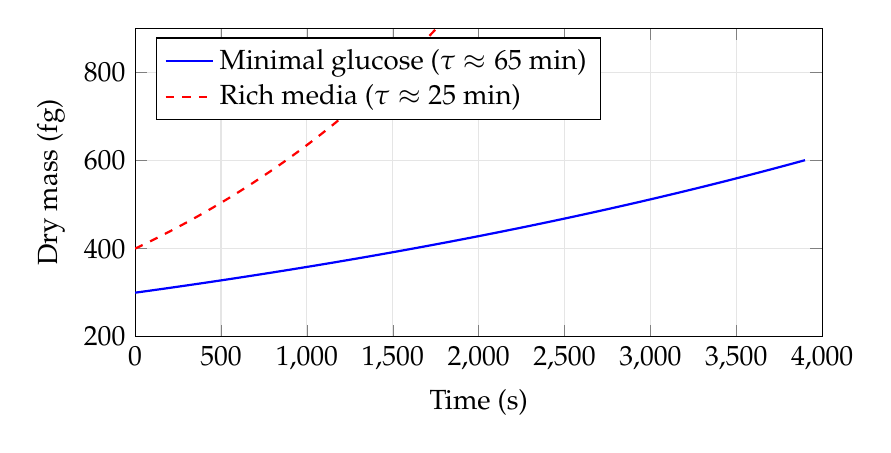
\begin{tikzpicture}
\begin{axis}[
    width=0.85\textwidth, height=5.5cm,
    xlabel={Time (s)},
    ylabel={Dry mass (fg)},
    legend pos=north west,
    grid=major,
    grid style={gray!20},
    xmin=0, xmax=4000,
    ymin=200, ymax=900,
    legend cell align=left,
]
% Minimal media: ~65 min doubling, starts ~300 fg, ends ~600 fg
\addplot[blue, thick, domain=0:3900, samples=80]
  {300 * exp(0.000178*x)};
\addlegendentry{Minimal glucose ($\tau \approx 65$ min)}

% Rich media: ~25 min doubling, starts ~400 fg, ends ~800+ fg faster
\addplot[red, thick, dashed, domain=0:2000, samples=60]
  {400 * exp(0.000462*x)};
\addlegendentry{Rich media ($\tau \approx 25$ min)}
\end{axis}
\end{tikzpicture}
\caption{Schematic dry mass trajectories for \textit{E.~coli} growing in
  minimal glucose medium (blue, solid) versus rich medium supplemented with
  amino acids (red, dashed).  The rich-media cell starts larger, grows
  faster, and divides sooner.  Curves are illustrative of the model output;
  actual traces include stochastic fluctuations.}
\label{fig:mass}
\end{figure}

\begin{figure}[H]
\centering
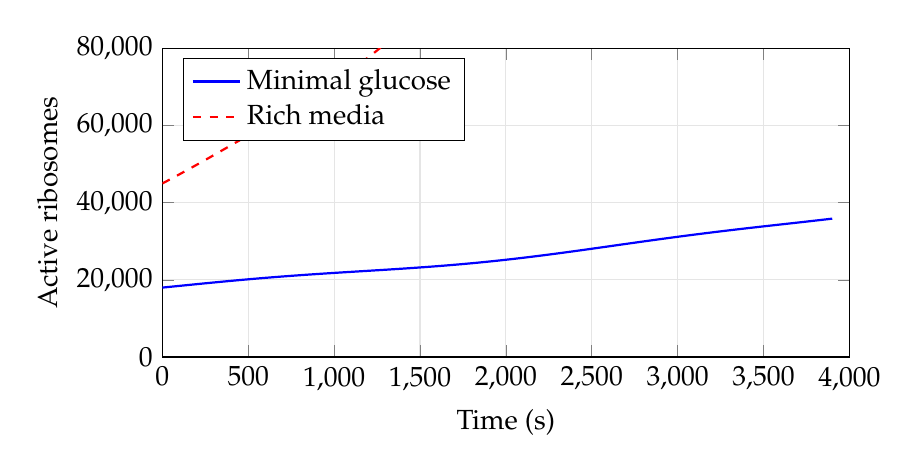
\begin{tikzpicture}
\begin{axis}[
    width=0.85\textwidth, height=5.5cm,
    xlabel={Time (s)},
    ylabel={Active ribosomes},
    legend pos=north west,
    grid=major,
    grid style={gray!20},
    xmin=0, xmax=4000,
    ymin=0, ymax=80000,
    legend cell align=left,
    scaled y ticks=false,
    yticklabel style={/pgf/number format/fixed},
]
% Minimal: ~15-20k ribosomes, growing slowly
\addplot[blue, thick, domain=0:3900, samples=80]
  {18000 * exp(0.000178*x) + 500*sin(deg(x/400))};
\addlegendentry{Minimal glucose}

% Rich: ~55k ribosomes, growing faster
\addplot[red, thick, dashed, domain=0:2000, samples=60]
  {45000 * exp(0.000462*x) + 800*sin(deg(x/300))};
\addlegendentry{Rich media}
\end{axis}
\end{tikzpicture}
\caption{Schematic active ribosome counts.  In rich media the cell invests a
  much larger fraction of its proteome in the translational machinery.  This
  is the ``growth law'' of Scott et al.~\cite{Scott2010}, reproduced here as
  an emergent prediction of the whole-cell model.}
\label{fig:ribosomes}
\end{figure}

Table~\ref{tab:conditions} summarises the key differences.  The model
captures all of these as consequences of its underlying biochemistry, not as
separate parameters.

\begin{table}[H]
\centering
\caption{Key simulation outputs for two growth conditions.}
\label{tab:conditions}
\begin{tabular}{lcc}
  \toprule
  \textbf{Metric} & \textbf{Minimal glucose} & \textbf{Rich media} \\
  \midrule
  Doubling time             & $\sim$65 min   & $\sim$25 min \\
  Initial dry mass          & $\sim$300 fg   & $\sim$400 fg \\
  Ribosomal protein fraction & $\sim$15--20\% & $\sim$35--40\% \\
  Biosynthetic enzyme fraction & $\sim$15\%  & $\sim$3--5\% \\
  RNA-to-protein ratio       & Lower          & Higher \\
  \bottomrule
\end{tabular}
\end{table}

The model also supports \emph{nutrient shift} experiments: a simulation can
begin in minimal medium and switch to rich medium (or vice versa) at a
specified time.  The resulting transient --- a burst of rapid growth as the
cell reallocates its resources --- matches experimental observations of
the stringent response~\cite{AhnHorst2022}.


% ══════════════════════════════════════════════════════════
\part{Architecture}
% ══════════════════════════════════════════════════════════

% ──────────────────────────────────────────────────────────
\section{Repository Structure}
% ──────────────────────────────────────────────────────────

The codebase is written in Python 3.11 with three performance-critical modules
compiled via Cython.  It is organised into three top-level packages, each with
a distinct role:

\begin{description}[style=nextline, leftmargin=2cm]
  \item[\texttt{wholecell/}]
    The \emph{generic simulation engine}.  Base classes for processes, states,
    listeners, and views; the simulation loop; binary I/O; a units library;
    and optional workflow orchestration (FireWorks).  This code is
    organism-agnostic.

  \item[\texttt{models/ecoli/}]
    The \textit{E.~coli}-specific model.  Seventeen process implementations,
    eighteen listener implementations, $\sim$32 variant definitions, and over
    80 analysis plot scripts.  Each is a subclass of a framework base class.

  \item[\texttt{reconstruction/ecoli/}]
    The Parameter Calculator (ParCa).  Reads $\sim$80 flat TSV files of raw
    experimental data and fits them into a single parameter object
    (\texttt{sim\_data}), serialised to disk.  The main orchestrator
    (\texttt{fit\_sim\_data\_1.py}) is $\sim$150\,KB of Python.
\end{description}

This separation is the key architectural insight: the framework is designed to
be reused for other organisms.

% ──────────────────────────────────────────────────────────
\section{The Simulation Loop}
\label{sec:simloop}
% ──────────────────────────────────────────────────────────

The simulation is driven by a fixed-timestep loop (default: 1 second).  Each
tick proceeds through five phases:

\begin{enumerate}[nosep]
  \item \textbf{Request.}  Each process calls \texttt{calculateRequest()} to
    declare how many of each molecule it would like to consume.
  \item \textbf{Partition.}  The \texttt{BulkMolecules} state divides the
    available integer counts among processes according to priority levels
    (e.g.\ metabolism at $-10$ gets first pick; degradation at $+10$ gets
    last).
  \item \textbf{Evolve.}  Each process calls \texttt{evolveState()} to update
    the cell's state using its allocated molecules.
  \item \textbf{Merge.}  Consumed and produced molecules are reconciled back
    into the global state.
  \item \textbf{Listen.}  Each listener reads the updated state (read-only)
    and appends one row to its output table.
\end{enumerate}

Processes run in \emph{dependency-ordered groups}.  Within a group, processes
share state and run in parallel; between groups, execution is sequential.  A
typical ordering is: TF unbinding $\to$ equilibrium $\to$ TF binding $\to$
transcription initiation $\to$ transcript/polypeptide elongation $\to$ \ldots
$\to$ cell division.

\begin{figure}[H]
\centering
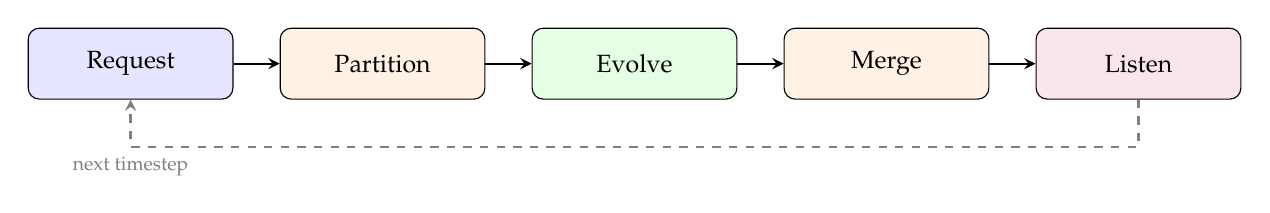
\begin{tikzpicture}[
    box/.style={draw, rounded corners, minimum height=0.9cm,
                minimum width=2.6cm, align=center, font=\small},
    arrow/.style={->, thick, >=stealth},
  ]
  \node[box, fill=blue!10]   (req)   at (0,0)    {Request};
  \node[box, fill=orange!10] (part)  at (3.2,0)  {Partition};
  \node[box, fill=green!10]  (evolve)at (6.4,0)  {Evolve};
  \node[box, fill=orange!10] (merge) at (9.6,0)  {Merge};
  \node[box, fill=purple!10] (listen)at (12.8,0) {Listen};

  \draw[arrow] (req)   -- (part);
  \draw[arrow] (part)  -- (evolve);
  \draw[arrow] (evolve)-- (merge);
  \draw[arrow] (merge) -- (listen);
  \draw[arrow, dashed, gray] (listen.south) -- ++(0,-0.6) -| (req.south)
    node[midway, below, font=\scriptsize\color{gray}] {next timestep};
\end{tikzpicture}
\caption{The five phases of each simulation timestep.}
\label{fig:loop}
\end{figure}

% ──────────────────────────────────────────────────────────
\section{Core Abstractions}
% ──────────────────────────────────────────────────────────

\subsection{Processes}

Every biological submodel is a subclass of
\texttt{wholecell.processes.process.Process}.  A process must implement:

\begin{lstlisting}
def initialize(self, sim, sim_data):
    """Set up references and constants from sim_data."""
def calculateRequest(self):
    """Declare molecule needs for this timestep."""
def evolveState(self):
    """Update cellular state using allocated molecules."""
\end{lstlisting}

Processes access the cell's state through \emph{views}:
\texttt{bulkMoleculesView} for integer counts of small molecules and
macromolecules; \texttt{uniqueMoleculesView} for individually tracked objects
(each ribosome, each replication fork); and \texttt{environmentView} for
external nutrient concentrations.

The 17 \textit{E.~coli} processes include metabolism (flux-balance analysis),
transcript initiation and elongation, polypeptide initiation and elongation,
chromosome replication and structure, transcription factor binding, RNA and
protein degradation, complexation, equilibrium, two-component signalling,
RNA maturation, and cell division.

\subsection{States}

Three state containers hold the cell's molecular inventory:

\begin{description}[nosep]
  \item[\texttt{BulkMolecules}] Integer counts of every molecular species,
    tagged by compartment (\texttt{[c]} cytoplasm, \texttt{[p]} periplasm,
    \texttt{[e]} extracellular).  The partitioning system divides these counts
    among processes each timestep.
  \item[\texttt{UniqueMolecules}] Individually tracked objects with per-instance
    attributes (e.g.\ a ribosome's position along an mRNA, a replication fork's
    chromosomal coordinate).
  \item[\texttt{LocalEnvironment}] External nutrient concentrations, supporting
    media-shift timelines.
\end{description}

\subsection{Listeners and Data I/O}

Listeners are read-only observers that record data each timestep.  Each listener
writes to a directory of zlib-compressed column files using a custom binary
format (\texttt{TableWriter}/\texttt{TableReader}).  The 18 \textit{E.~coli}
listeners record mass fractions, metabolic fluxes, ribosome data, replication
progress, and more.

Simulation output is stored in a hierarchical directory structure:

\begin{Verbatim}[fontsize=\small]
out/<sim_dir>/
  kb/simData                     # Fitted parameters
  <variant>_<index>/             # e.g. wildtype_000000/
    <seed>/                      # e.g. 000000/
      generation_<gen>/
        <daughter>/
          simOut/                 # Listener data (TableWriter)
          plotOut/                # Analysis figures
\end{Verbatim}

Reading data back requires the \texttt{TableReader} class:

\begin{lstlisting}
from wholecell.io.tablereader import TableReader
reader = TableReader(os.path.join(simout, 'Mass'))
dry_mass = reader.readColumn('dryMass')
\end{lstlisting}

\subsection{Units}

Physical quantities carry units throughout the codebase via the \texttt{Unum}
library.  A value is stripped of its units only at the point of computation:

\begin{lstlisting}
from wholecell.utils import units
conc = 100 * units.mmol / units.L
value = conc.asNumber(units.mol / units.L)  # -> 0.1
\end{lstlisting}


% ══════════════════════════════════════════════════════════
\part{The Web Interface}
% ══════════════════════════════════════════════════════════

% ──────────────────────────────────────────────────────────
\section{Motivation}
% ──────────────────────────────────────────────────────────

The standard way to use wcEcoli is from the command line.  A researcher
wishing to run a simulation must type a series of Python commands, wait for
them to finish, and then run separate analysis scripts to produce plots.
Inspecting specific data columns requires writing short Python scripts using a
custom binary data reader.

To lower this barrier, I have built a browser-based user interface (the
``webapp'') that wraps the existing model with four interactive tabs:

\begin{description}[style=nextline, leftmargin=1.5cm]
  \item[Configure]
    A form with quick-start presets (e.g.\ ``Wildtype baseline,''
    ``Nutrient upshift,'' ``Rich media'') and full control over variant
    type, number of generations, random seeds, and regulation toggles.
    Clicking \emph{Run Simulation} submits the job to a background queue.

  \item[Run Status]
    A live-updating table showing each submitted job, its current phase
    (parameter fitting, simulating, analysing), and elapsed time.

  \item[Inspect Data]
    An interactive chart that lets the user browse any listener and any
    data column from any completed run.  Multiple runs can be overlaid on
    the same graph for comparison.  Transforms (normalisation, log scale)
    are available as checkboxes.

  \item[Explore Plots]
    A gallery of the pre-generated analysis plots (the same 80+ scripts
    mentioned earlier), with side-by-side comparison of two runs.
\end{description}

The practical benefit is that a researcher who is not a software developer
can configure, run, and inspect simulations entirely from a web browser.

% ──────────────────────────────────────────────────────────
\section{Technology and Architecture}
% ──────────────────────────────────────────────────────────

The web interface is a \textbf{Dash} application (Plotly's reactive web
framework, built on Flask).  It runs as a single Python process, serves a
browser UI on \texttt{localhost}, and interacts with the simulation code
through the same Python API that the command-line scripts use.

Key dependencies: Dash 2.9, Plotly 5.14, Flask (via Dash).  The application
is containerised via Docker for deployment to Azure Container Instances, with
CI/CD via GitHub Actions.

The codebase is organised as follows:

\begin{description}[style=nextline, leftmargin=2cm]
  \item[\texttt{app.py}]
    The application factory.  Creates the Dash app, builds all four tab layouts
    upfront (so every component ID is registered in the initial layout), wires
    tab-switching via CSS \texttt{display} toggling, and registers each tab's
    callbacks.

  \item[\texttt{results.py}]
    Data-access layer.  Functions to scan the \texttt{out/} directory tree for
    simulation runs, variants, cells, listeners, and columns.  Also provides
    the \texttt{load\_column()} and \texttt{load\_time()} functions that wrap
    \texttt{TableReader}.

  \item[\texttt{jobs.py}]
    A SQLite-backed job queue.  A background thread picks up queued jobs and
    runs them as subprocesses (either local Python or Docker containers),
    stepping through phases: queued $\to$ parca $\to$ simulating $\to$
    analysing $\to$ done/failed.

  \item[\texttt{tabs/}]
    Four tab modules, each exporting a \texttt{layout()} function and a
    \texttt{register\_callbacks()} function:
    \begin{itemize}[nosep]
      \item \texttt{inspect\_data.py} --- interactive listener data browser
      \item \texttt{explore.py} --- analysis plot gallery with side-by-side
            comparison
      \item \texttt{configure.py} --- simulation setup form with presets
      \item \texttt{runs.py} --- live job-queue monitor
    \end{itemize}
\end{description}

\subsection{The Inspect Data tab in detail}

This is the most complex tab.  Its callback graph demonstrates how reactive
state management works in Dash:

\begin{enumerate}[nosep]
  \item \textbf{Run dropdown} $\to$ populates Listener dropdown (defaults to
    \texttt{Mass}).
  \item \textbf{Listener dropdown} $\to$ populates Column dropdown (defaults to
    \texttt{dryMass} for Mass, \texttt{time} for Main).
  \item \textbf{Column selection + transforms + overlay store} $\to$ renders the
    Plotly figure with primary trace (solid line) and any overlay traces (dashed
    lines).
  \item \textbf{Overlay panel}: cascading Run/Listener/Column dropdowns $\to$
    ``Add Trace'' button appends to a \texttt{dcc.Store} $\to$ triggers graph
    re-render.  Each added trace is listed below the panel with a remove button.
  \item \textbf{Delete button} $\to$ \texttt{dcc.ConfirmDialog} $\to$ on
    confirm, removes the variant directory from disk; all dropdown
    options across both Inspect and Explore tabs are refreshed.
\end{enumerate}

Overlay traces use Dash \emph{pattern-matching callbacks}
(\texttt{\{``type'': ``remove-overlay-trace'', ``index'': ALL\}}) to handle a
dynamic number of remove buttons without pre-registering each one.

When a run is deleted from the Inspect tab, the callback must also update the
Explore tab's dropdown options and selected values.  This is handled by a
single callback with outputs spanning both tabs.  Shared utility functions
live in \texttt{results.py} to avoid cross-tab imports.


% ══════════════════════════════════════════════════════════
\part{Proposed Extension: Whole-Cell Platelet Model}
% ══════════════════════════════════════════════════════════

% ──────────────────────────────────────────────────────────
\section{Biological Motivation}
% ──────────────────────────────────────────────────────────

Human platelets are anucleate blood cells responsible for haemostasis.  They
circulate for 7--10 days in a resting state, become activated at sites of
vascular injury, and respond by releasing granule contents, changing shape,
and aggregating.  Despite their clinical importance --- they are central to
both bleeding disorders and thrombotic disease --- no whole-cell model of a
platelet exists.  Current models focus on individual pathways (calcium
signalling, integrin activation, coagulation cascades) but do not integrate
them.

\subsection{How platelets differ from \textit{E.~coli}}

The modelling challenges are quite different from those of a bacterium:

\begin{itemize}[nosep]
  \item \textbf{No genome, no division.}  Platelets have no nucleus.  There
        is no DNA replication, no transcription from a genome, and no cell
        division.  The relevant timescale is a \emph{lifespan} (7--10 days),
        not a cell cycle.
  \item \textbf{Activation, not growth.}  The interesting biology is not
        steady-state growth but a transition: resting $\to$ primed $\to$
        activated $\to$ spent.  This happens over seconds to minutes.
  \item \textbf{Compartments matter.}  Platelets contain dense granules,
        alpha-granules, an open canalicular system, and mitochondria.
        Trafficking between these compartments is central to platelet
        function.
  \item \textbf{Calcium as the central integrator.}  Receptor signalling
        converges on intracellular calcium concentration, which in turn
        triggers granule release and integrin activation.
\end{itemize}


% ──────────────────────────────────────────────────────────
\section{Framework Reusability Analysis}
\label{sec:reuse}
% ──────────────────────────────────────────────────────────

I have conducted a detailed analysis of every wcEcoli component to assess
reusability.  The results are summarised in Table~\ref{tab:reuse}.

\begin{table}[H]
\centering
\caption{Reusability of wcEcoli components for a platelet model.}
\label{tab:reuse}
\small
\begin{tabular}{llp{6cm}}
  \toprule
  \textbf{Component} & \textbf{Verdict} & \textbf{Action} \\
  \midrule
  \texttt{Simulation} loop       & Fully generic & Subclass \\
  \texttt{Process} base class    & Fully generic & Use as-is \\
  \texttt{View} abstractions     & Fully generic & Use as-is \\
  \texttt{InternalState} base    & Fully generic & Use as-is \\
  \texttt{Listener} base class   & Fully generic & Use as-is \\
  \texttt{TableWriter/Reader}    & Fully generic & Use as-is \\
  \texttt{BulkMolecules}         & Mostly generic & Override one
    hardcoded ATP reference \\
  \texttt{UniqueMolecules}       & Mostly generic & Generalise
    compartment mass calculation \\
  \texttt{LocalEnvironment}      & Mostly generic & Map media timeline
    to agonist-addition timeline \\
  \texttt{divide\_cell.py}       & Not needed & Platelets do not divide \\
  \texttt{models/ecoli/*}        & Not reusable & Write new platelet code \\
  \texttt{reconstruction/ecoli/} & Not reusable & Write new parameter set \\
  Web UI                         & Fully reusable & Works with any organism \\
  \bottomrule
\end{tabular}
\end{table}

\subsection{Key engine modifications needed}

\begin{itemize}[nosep]
  \item \textbf{Termination condition.}  The simulation currently ends when the
    cell divides.  For platelets, it should terminate on a time limit or a
    biological condition (e.g.\ complete degranulation).  Setting
    \texttt{\_raise\_on\_time\_limit = False} in the simulation subclass
    achieves this.
  \item \textbf{No division function.}  Simply never setting
    \texttt{\_divideCellFunction} is sufficient; the engine handles this
    gracefully.
  \item \textbf{Compartment mass.}  \texttt{UniqueMolecules.calculateMass()}
    hardcodes compartment \texttt{`c'}.  This needs generalisation for a
    multi-compartment platelet model (cytosol, dense granules, alpha granules,
    mitochondria).
\end{itemize}


% ──────────────────────────────────────────────────────────
\section{Data Requirements}
\label{sec:data}
% ──────────────────────────────────────────────────────────

A whole-cell model is only as good as the data used to parameterise it.
Two published datasets are particularly important for a platelet model:

\begin{description}[style=nextline, leftmargin=0.5cm]
  \item[Burkhart et al.\ (2012)~\cite{Burkhart2012}]
    The first comprehensive quantitative proteome of human platelets, covering
    over 4\,000 proteins with copy-number estimates.  This dataset would serve
    a role analogous to that of EcoCyc in the \textit{E.~coli} model: it
    provides the initial molecular inventory (what is present and in what
    quantity) from which to derive initial conditions, enzyme concentrations,
    and receptor densities.  It also enables comparative analysis of structural
    and functional pathways, which is essential for deciding which processes to
    include and how to parameterise them.

  \item[Purvis et al.\ (2008)~\cite{Purvis2008}]
    A molecular signalling model of platelet phosphoinositide and calcium
    regulation, covering both resting homeostasis and P2Y$_1$ receptor
    activation.  This paper provides ODE rate constants, calcium store
    capacities, and IP$_3$-mediated release kinetics --- exactly the
    quantitative parameters needed to implement the calcium dynamics process.
    It also serves as a validation target: the platelet model's calcium
    transients should reproduce the profiles reported in this work.
\end{description}

Additional data sources will be needed as the model grows (e.g.\ granule
secretion kinetics from lumiaggregometry studies, integrin affinity
measurements), but these two papers provide the essential foundation for the
initial phases described below.


% ──────────────────────────────────────────────────────────
\section{Proposed File Structure}
% ──────────────────────────────────────────────────────────

\begin{Verbatim}[fontsize=\small]
models/platelet/
    sim/
        simulation.py             # PlateletSimulation(Simulation)
        initial_conditions.py
    processes/
        calcium_dynamics.py       # Store release, influx, buffering
        granule_release.py        # Dense/alpha granule exocytosis
        receptor_signalling.py    # GPVI, PAR, P2Y12 -> Ca2+
        protein_decay.py          # Slow mRNA/protein turnover
    listeners/
        mass.py
        calcium.py
        granule_state.py
    analysis/
        single/
            calcium_trace.py
            granule_secretion.py
reconstruction/platelet/
    simulation_data.py            # SimulationDataPlatelet
    knowledge_base_raw.py
    dataclasses/
        constants.py
        molecule_groups.py
\end{Verbatim}


% ──────────────────────────────────────────────────────────
\section{Implementation Ideas}
\label{sec:plan}
% ──────────────────────────────────────────────────────────

The following outlines a phased approach to building the platelet model.
These are ideas for future work; the scope of the project is limited and
time will likely only allow some of these to be tackled.  I present them
here to show the range of what is possible and to provide a roadmap that
could be followed incrementally.

\subsection{Phase 1: Understand the engine}

Run the \textit{E.~coli} model end-to-end.  Trace the simulation loop,
document the interfaces that a new organism must satisfy, and identify the
minimum \texttt{sim\_data} contract.  The key interface points are:

\begin{itemize}[nosep]
  \item \texttt{submass\_name\_to\_index} and
    \texttt{compartment\_abbrev\_to\_index} (mass accounting)
  \item \texttt{constants.n\_avogadro} (unit conversions)
  \item \texttt{internal\_state.bulk\_molecules.bulk\_data} (molecule IDs and
    masses)
  \item \texttt{internal\_state.unique\_molecule.unique\_molecule\_definitions}
    (can be empty)
  \item \texttt{molecule\_groups.*\_division} (can be empty lists for a
    non-dividing cell)
\end{itemize}

\emph{Deliverable:} a short architecture document.

\subsection{Phase 2: Build a minimal platelet stub}

Create \texttt{models/platelet/} with one process (e.g.\
\texttt{RestingDecay}), one listener (\texttt{Mass}), and a skeleton
\texttt{SimulationDataPlatelet}.  The goal is a simulation that runs, produces
output visible in the web UI, and provides a scaffold for incremental
development.  The initial molecular inventory would draw on copy-number
estimates from Burkhart et al.~\cite{Burkhart2012}.

Estimated scope: $\sim$500 lines of new code.

\emph{Deliverable:} a runnable platelet stub.

\subsection{Phase 3: Add biology incrementally}

Each of the following items represents a self-contained extension.  They are
listed in a logical order of dependency, but any subset could be implemented
independently depending on available time:

\begin{enumerate}
  \item \textbf{Calcium dynamics.}  Model calcium stores (dense tubular system)
    with release via IP$_3$ receptors, plasma-membrane influx (store-operated
    calcium entry), and cytosolic buffering.  Mathematical formalism: ODEs,
    similar to the tRNA-charging solver already in the \textit{E.~coli}
    model.  Rate constants and store capacities would be drawn from Purvis
    et al.~\cite{Purvis2008}, and the resulting calcium transients could be
    validated against the same paper's reported profiles.

  \item \textbf{Granule release.}  Dense granules and alpha granules as
    \texttt{UniqueMolecule} instances, each with a state attribute (loaded,
    fusing, released).  Exocytosis is triggered stochastically when
    cytosolic calcium exceeds a threshold, at a rate proportional to
    $[\text{Ca}^{2+}]$.  Cargo (ADP, serotonin, fibrinogen, vWF) moves from
    granule to extracellular compartment.

  \item \textbf{Receptor signalling.}  Coarse-grained models of the three
    major activation pathways:
    \begin{itemize}[nosep]
      \item GPVI (collagen receptor) $\to$ PLC$\gamma$2 $\to$ IP$_3$ $\to$
            Ca$^{2+}$ release
      \item PAR-1/4 (thrombin receptors) $\to$ PLC$\beta$ $\to$ IP$_3$ $\to$
            Ca$^{2+}$ release
      \item P2Y$_{12}$ (ADP receptor) $\to$ inhibition of adenylyl cyclase
            $\to$ amplification of activation
    \end{itemize}

  \item \textbf{Integrin activation} (optional).  $\alpha$IIb$\beta$3
    inside-out signalling, fibrinogen binding, outside-in signalling.

  \item \textbf{Metabolism} (optional).  Mitochondrial ATP production,
    glycolysis.  Lower priority because energy depletion is not the primary
    driver of acute platelet activation.
\end{enumerate}

\emph{Deliverable (if time allows):} a version~0.1 model simulating
thrombin-induced calcium rise and dense-granule release over five minutes,
with secretion kinetics plots.

\subsection{Why start with granule release?}

Three reasons:

\begin{enumerate}[nosep]
  \item Granules are \emph{discrete, countable objects} --- a natural fit for
    the \texttt{UniqueMolecules} state, which already tracks individual
    ribosomes and replication forks in the \textit{E.~coli} model.
  \item Granule release has \emph{clear experimental observables}: ATP/ADP
    secretion profiles, serotonin release kinetics, P-selectin surface
    expression (measurable by flow cytometry).
  \item It \emph{bridges multiple scales}: receptor binding (molecular) $\to$
    calcium signalling (pathway) $\to$ exocytosis (organelle) $\to$
    extracellular cargo (cell-level output).  This is exactly the kind of
    multi-scale integration that a whole-cell model is designed for.
\end{enumerate}


% ══════════════════════════════════════════════════════════
\section*{Summary}
% ══════════════════════════════════════════════════════════

The wcEcoli whole-cell model is a mature, open-source simulation of
\textit{E.~coli} that integrates 17 biological processes and reproduces
emergent properties such as growth-rate-dependent ribosome allocation.  I
have built a web interface that makes it accessible to non-programmers, and I
propose to reuse its generic simulation engine to explore the feasibility of
building the first whole-cell model of a human platelet, starting with calcium
dynamics and granule release.  The scope of the proposed work is ambitious;
the phased approach allows meaningful progress even if only the earlier stages
are completed within the available time.


% ══════════════════════════════════════════════════════════
\section*{Use of Artificial Intelligence}
% ══════════════════════════════════════════════════════════

This report, the web interface, and supporting code were developed with
substantial assistance from AI tools.  Specifically:

\begin{itemize}[nosep]
  \item \textbf{GitHub Copilot} was used throughout the development of the web
    interface for code completion, boilerplate generation, and exploratory
    prototyping.
  \item \textbf{Claude Code} (Anthropic's Claude, via the CLI tool) was used
    for code review, refactoring, architectural analysis of the wcEcoli
    framework, and generating this report document.
\end{itemize}

All AI-generated code was reviewed, tested, and modified by the author before
inclusion.  The biological content and proposed modelling strategy reflect the
author's own analysis, informed by the referenced literature, though the prose
was drafted with AI assistance and then edited for accuracy and style.

I believe transparency about AI usage is important.  These tools significantly
accelerated development --- particularly for the web interface and for
navigating the large wcEcoli codebase --- but the scientific judgements,
architectural decisions, and biological reasoning are my own.

\vspace{1em}
\printbibliography

\end{document}
